\subsection{Design Choices and Sensitivity}
\label{sec:exp-design}

We now justify NESS's design choices and show that its performance is not brittle to hyperparameters. All studies are on ogbn-arxiv at $80\%$ missingness.

\paragraph{Design choices.} Figure~\ref{fig:design} compares the two principal architectural decisions, each varied in isolation. For the encoder, GraphSAGE outperforms GAT and GCN; its separate self-transformation preserves each node's prefilled signal through depth, which a mean-based aggregator does not. For the prefill, Feature Propagation clearly beats a single round of neighbor-mean imputation and zero-filling, confirming that long-range diffusion recovers signal that a single aggregation step or no imputation cannot. (The two panels are separate ablations and share only the metric axis; absolute values are not directly comparable across them.)

\paragraph{Component ablation.} Table~\ref{tab:components} removes NESS's learning components one at a time. Removing the self-supervised objectives (no-SSL) and, more so, the entire two-view contrastive structure (single-view) both reduce performance, and removing the Feature-Propagation prefill (zero-fill) is the most damaging. Each component contributes, and the prefill is the single most important.

\paragraph{Hyperparameter sensitivity.} Figure~\ref{fig:hp} varies four hyperparameters one at a time around the chosen configuration. Performance is stable and peaks near the selected values: a deeper (three-layer) encoder and lower dropout ($0.3$) are preferable, and the learning rate is stable around $10^{-3}$. Up-weighting the classification term improves results and then plateaus; we set its weight to $3$, a stable point on this plateau rather than the extreme, to avoid over-emphasizing the supervised term at the expense of the auxiliary signal that matters at higher missingness.

\begin{figure}[t]
\centering
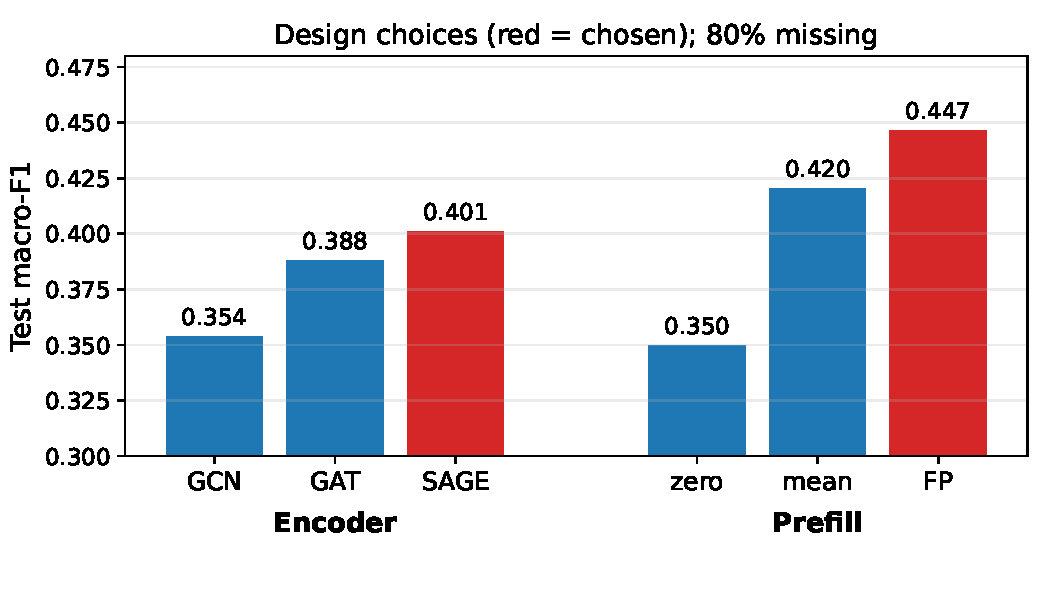
\includegraphics[width=\linewidth]{figures/e11_design_choices.pdf}
\caption{Design choices (chosen option in red), on ogbn-arxiv at $80\%$ missingness. GraphSAGE is the best encoder and Feature Propagation the best prefill. The two panels are independent ablations.}
\label{fig:design}
\end{figure}

\begin{figure}[t]
\centering
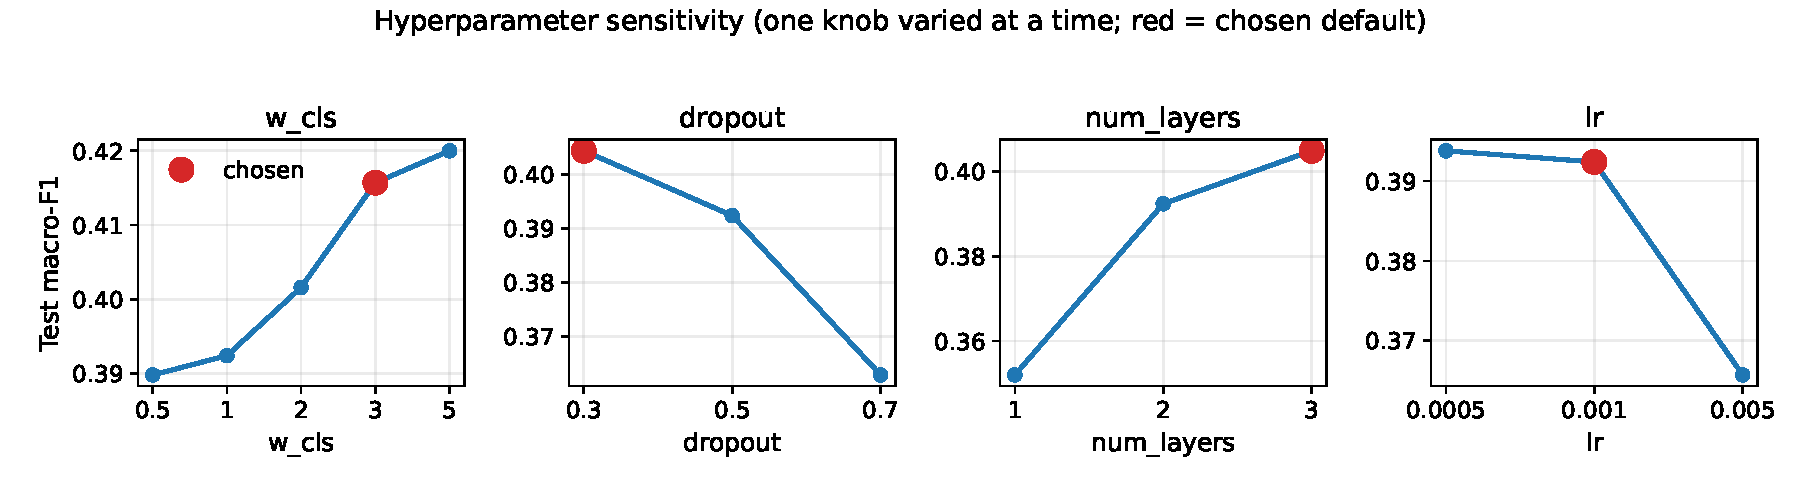
\includegraphics[width=\linewidth]{figures/e11_hp_sensitivity.pdf}
\caption{Hyperparameter sensitivity: each knob is varied with the others fixed; the chosen default is marked in red. Performance is stable and peaks near the selected settings.}
\label{fig:hp}
\end{figure}

\begin{table}[t]
\centering
\caption{Component ablation on ogbn-arxiv at $80\%$ missingness (test macro-F1, three seeds). Removing any learning component reduces performance; the prefill matters most.}
\label{tab:components}
\small
\begin{tabular}{@{}lc@{}}
\toprule
\textbf{Configuration} & \textbf{Test F1} \\
\midrule
NESS (full)                       & \textbf{0.447} \\
\;\; without SSL objectives       & 0.424 \\
\;\; without two-view contrastive & 0.416 \\
\;\; without FP prefill (zero-fill) & 0.350 \\
\bottomrule
\end{tabular}
\end{table}
